\documentclass[11pt,twocolumn]{article}
\usepackage{graphicx}
\graphicspath{ {../img/} }
\title{
        
\includegraphics{logo/vertical_black} \\
        \large A trading card game on the Ethereum Blockchain
        }
\author{DRAFT}
\date{\today}

\usepackage{tikz}
\usepackage{pgfplots}
\usepackage{filecontents}

\begin{filecontents}{datax.dat}
        0,16124
        1,16349
        2,16365
        3,16410
        4,16551
        5,16491
        6,16772
        7,16762
        8,16752
        9,16961
        10,16837
        11,17078
        12,17127
        13,17165
        14,17299
        15,17214
        16,17534
        17,17489
        18,17583
        19,17569
        20,17531
        21,17782
        22,17742
        23,17835
        24,17886
        25,17908
        26,18161
        27,18196
        28,18397
        29,18372
        30,18336
        31,18649
        32,18775
        33,18967
        34,18929
        35,18832
        36,19044
        37,19349
        38,19475
        39,19445
        40,19276
        41,19534
        42,19675
        43,19780
        44,19738
        45,19640
        46,19940
        47,20105
        48,20175
        49,20189
        50,3917
        51,3522
        52,3619
        53,3659
        54,3607
        55,3507
        56,3158
        57,3334
        58,3292
        59,3175
        60,3108
        61,2765
        62,2803
        63,2828
        64,2777
        65,2754
        66,2370
        67,2535
        68,2424
        69,2367
        70,2342
        71,1961
        72,2033
        73,1992
        74,1967
        75,1962
        76,1592
        77,1642
        78,1667
        79,1537
        80,1614
        81,1240
        82,1211
        83,1230
        84,1249
        85,1134
        86,789
        87,825
        88,813
        89,793
        90,802
        91,398
        92,383
        93,392
        94,406
        95,410
    \end{filecontents}
    
\begin{document}
\maketitle

\twocolumn
\pagebreak
\pagebreak
\hspace*{-1.3in}
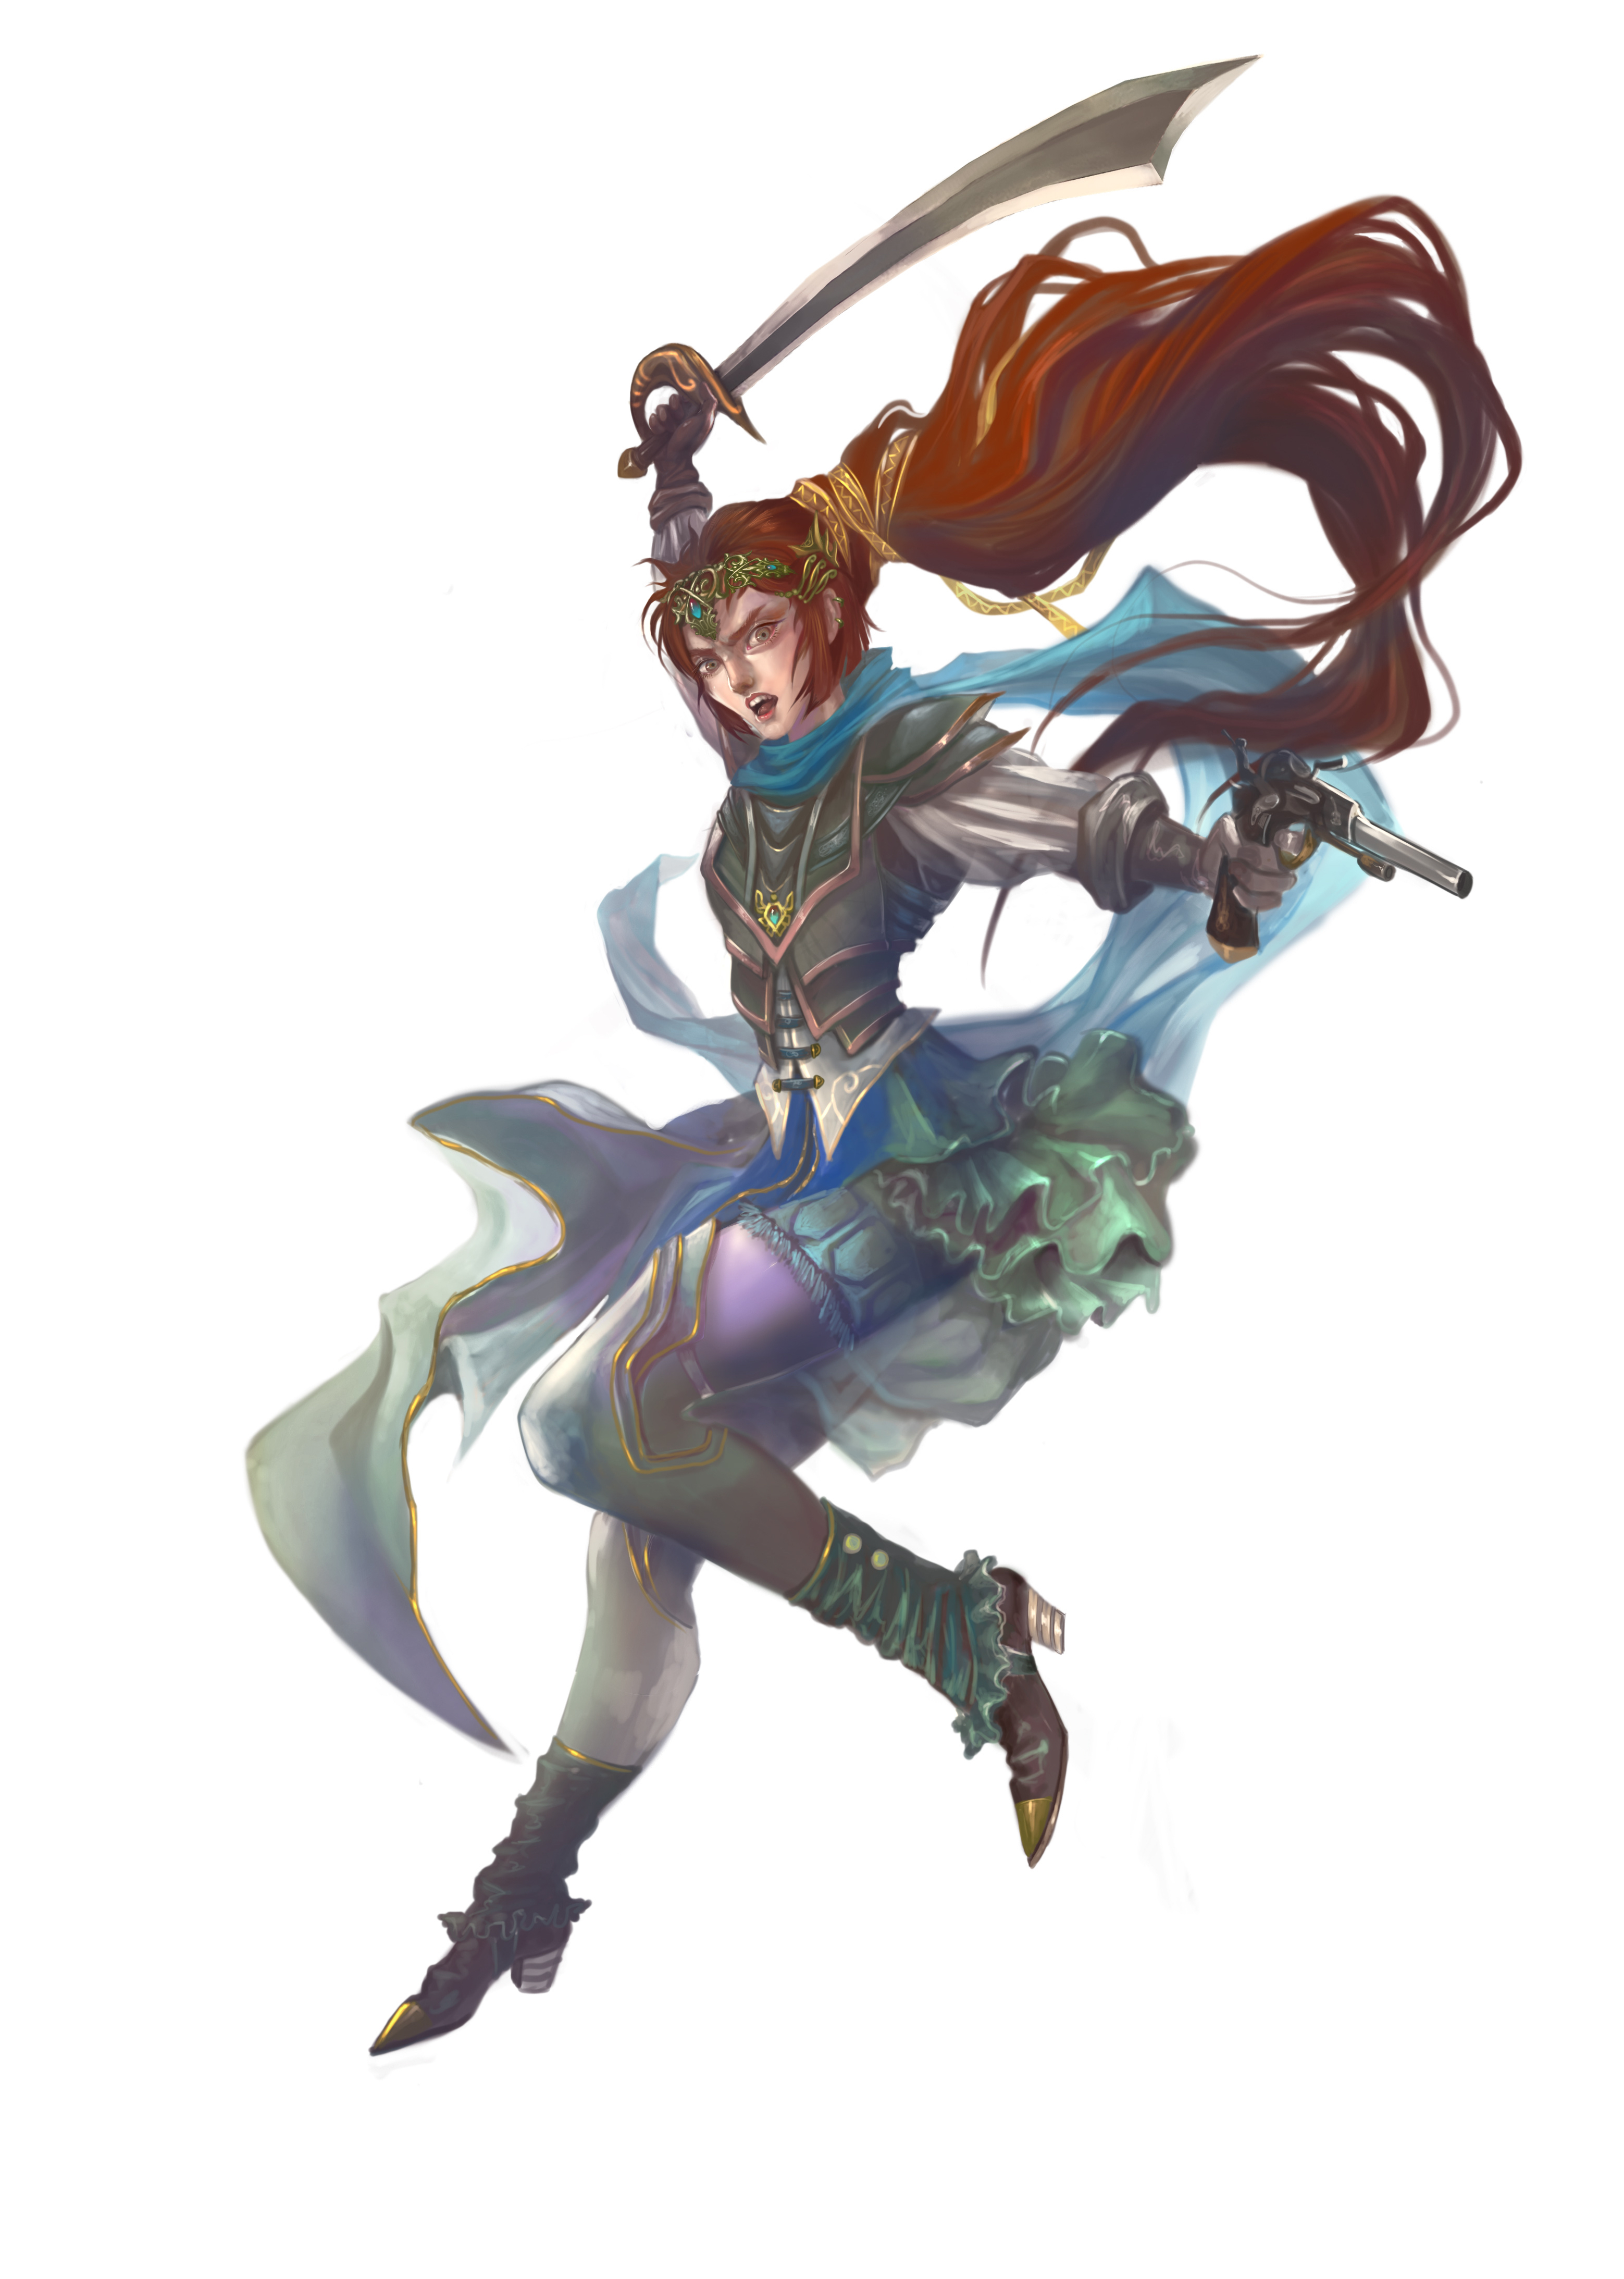
\includegraphics[scale=0.1]{art/princess} \\
\pagebreak
\section{Introduction}
\begin{quote}"I happily played World of Warcraft during 2007-2010, but one day Blizzard removed the damage component from my beloved warlock's Siphon Life spell. I cried myself to sleep, and on that day I realized what horrors centralized services can bring."
        \begin{flushright}
                {---Vitalik Buterin, Creator of Ethereum}
              \end{flushright}
        \end{quote}

Collectible card games have existed in popular demand since decades. After the massification of the Internet, many of them were successfully digitized like \textit{Magic: The Gathering} and \textit{Pokemon} and new ones were created emulating the look and feel of the physical collectibles in form of a multiplayer videogame.
However, being of electronic nature, it's physical existence is an entry on a database, and the amount of each card each player owns is a counter inside a central server. Using databases to create trading card games can produce a fun experience at the cost of conceptual problems:

\begin{itemize}
        \item Only the owner of the software can allow/deny the use of the digital card within it's ecosystem.
        \item The digital card existence depends on the game systems to be online.
        \item The game owner can prohibit trading or markets for cards, which is usually enforced.
        \item The game owner can control the issuance of cards witout transparency to the user.
\end{itemize}

Thanks to Blockchain technology we can make a trading card game where all cards are stored in a Ethereum smart contract, where players obtain true ownership of the game object and are free to trade in an outside the game program.\\

By being a blockchain asset, each card will have the following qualities:

\begin{itemize}
        \item It's securely stored in an Ethereum wallet.
        \item The owner and only the owner has perpetual rights for transfer, trade or sale of the token
        \item It can be read by other applications, like a mobile wallet for ERC721 tokens.
        \item It's existence doesn't depend on the availability of the game owner systems.
\end{itemize}

Each card is composed of a serial number and a model id that corresponds to a card model. There can be many cards of the same model, with different serial numbers. Card models are contain metadata for it's appearance (an image file) and it's game action properties (ex: deals 3 damage points to enemy target).\\

The smart contract also controls immutable rules on the issuance of cards, including the total limit of cards to be issued and the rarity of card models.


\section{The Game}
Darkwinds is an online trading card game where two players confront each other in a sea battle of ships.\\

While the smart contract handles the ownership of tokens, game matches occur off-chain, in a webGL website running the Metamask web extension or compatible thin wallets. A game server is responsible for matchmaking between two adversaries, validating the signature of both players, thus verfying the ownership of both player decks. While the official game server will be the only endorsed way of playing Darkwinds, other developers are free to read the ABIs and access players cards to create different game modes, tournaments or applications that connect to the game.\\

Game servers only require a signed message from the user wallet to verify ownership. The user private keys are never read or stored.


\section{Anatomy of a Darkwinds token}
The card smart contract performs all the functions according to the ERC721 \cite{notes} standard. The cards are generated with a payable function called getBoosterPack and the amount of cards returned to the owner is determined by the price of cards, which is set by the owner using the setCardPrice function
\subsection{getCard}
Gets all the metadata for the card relevant to the game mechanics (actions, cost of invocation, effects, etc.)
\subsection{getBoosterPack}
Spends a determined amount of ETH to get a booster pack. Normally it will contain 10, 25 or 50 cards but the contract can be excecuted for a specific amount of cards multiplying the desired amount of cards with the cost.
\subsection{changeCardCost}
A function designed for the owner to change the price of the card, and by consequence the price of booster packs. By default is 1 finney.
\section{Card Generation}
Cards are generated with a KECCAK-256 operation on the last block timestamp and a modulo operation of 50. Every 5 cards we add another 50 modulo on the contract nonce in attempt to make a rare card. If both modulo operations are larger than 25, a rare card appears. The higher the model ID, the rarer the card is as shown in Figure A.

While it's possible to determine exactly when cards are being released, efforts are probably not practical. 

The smart contract stops generating cards when the hard cap of 1,000,000 is reached.
\begin{figure}[!htb]
\centering 
    
\begin{tikzpicture}
\begin{axis}[xlabel={Card Model},  scaled y ticks=base 10:-3,
        ytick scale label code/.code={},
        yticklabel={\pgfmathprintnumber{\tick}.000}]

% Graph column 2 versus column 0
\addplot table[x index=0,y index=1,col sep=comma] {datax.dat};


\end{axis}
\end{tikzpicture}
\caption{Distribution of 1 million cards estimated by a Monte Carlo simulation} \label{fig:A}
\end{figure}


\onecolumn

\begin{thebibliography}{1}

        \bibitem{notes} The ERC721 non-fungible token standard. https://github.com/ethereum/eips/issues/721, Dieter Shirley, 2017.
      
        \end{thebibliography}
\end{document}